%\documentclass[10pt,a4paper,slovene,openany]{book}
\documentclass[oneside,a4paper,openany,12pt]{scrbook}
%\usepackage[a4,center,cam]{crop}
%\usepackage[slovene]{babel}
%\usepackage[T1]{fontenc}
%\usepackage[pdftex]{graphicx,thumbpdf}
%\usepackage{epstopdf}
%\usepackage[math]{kurier}

\newcommand {\e}[1]{\mathrm{~#1}}
\usepackage{paralist}

%\setlength{\parskip}{1em}%
\setlength{\parindent}{0cm}

\usepackage{titling}
\usepackage{amsmath,amssymb,amsfonts,nicefrac}
\usepackage{graphicx}
\usepackage{color}
\usepackage{float}
\usepackage{mathtools}
\allowdisplaybreaks
\usepackage[pdftex,colorlinks=true,citecolor=blue,linkcolor=black,urlcolor=blue,bookmarks=true]{hyperref}
\usepackage{pifont}
\usepackage{dictsym}
\usepackage{braket}
\usepackage{slashed}
\DeclareMathOperator{\arcsinh}{arcsinh}
\include{definicije}
\usepackage{enumerate}

%\usepackage[utf8]{inputenc}
%\usepackage[titles]{tocloft}
%\usepackage{setspace}

\usepackage{xr}
\externaldocument{chapterI}

%
%
\title{\huge {Measurement of the decay $B \to KK\ell\nu$}}
\author{Matic Lubej}
%
%
\begin{document}
%\maketitle
\date{Ljubljana, 2018}
\begin{titlingpage} %This starts the title page
\begin{center}
%\includegraphics[scale=1]{slike/fmf.pdf}

%\begin{large}
%\vspace{2.5cm}
\textbf{\thetitle}\\
%\vspace{0.5 cm} 
\theauthor \\
%\end{large}
\vspace{0cm}
\thedate
\end{center}
\end{titlingpage}

\pagestyle{plain}
\pagenumbering{roman}

\chapter*{Changelog}

\tableofcontents
\addtocontents{toc}{~\hfill\textbf{Page}\par}

\pagenumbering{arabic}
\chapter{Introduction}

test
\chapter{Data and MC}

test
%\chapter{Event reconstruction}

test

\chapter{Event reconstruction}

In this chapter the procedure for event reconstruction of the decay Decay is shown, starting from final state particle selection and combining particles up the chain all the way to the $B$ meson. 

\section{Final state particles selection}

Since the neutrino escapes detection, we can only reconstruct the charged tracks of our decay, which are the two kaons ($K$) and the light lepton, which is the electron ($e$) or muon ($\mu$). These are some of the particles which are commonly referred to as final state particles (FSP). Final state particles have a long lifetime and are usually the particles that we detect when they interact with the material in the detector.

It is important to limit our selection of FSP particles in order to cut down the number of particle combinations and to reduce computation time and file sizes.

\subsubsection{Leptons}

The following plots show the impact parameters $d_0$ and $z_0$, the momentum in  $\Upsilon(4S)$ center-of-mass system (CMS), and the $K/\pi$ PID information for true and fake electrons and muons, where an extra category for true electrons/muons from the signal decay is shown.

\begin{figure}[!h]
\centering
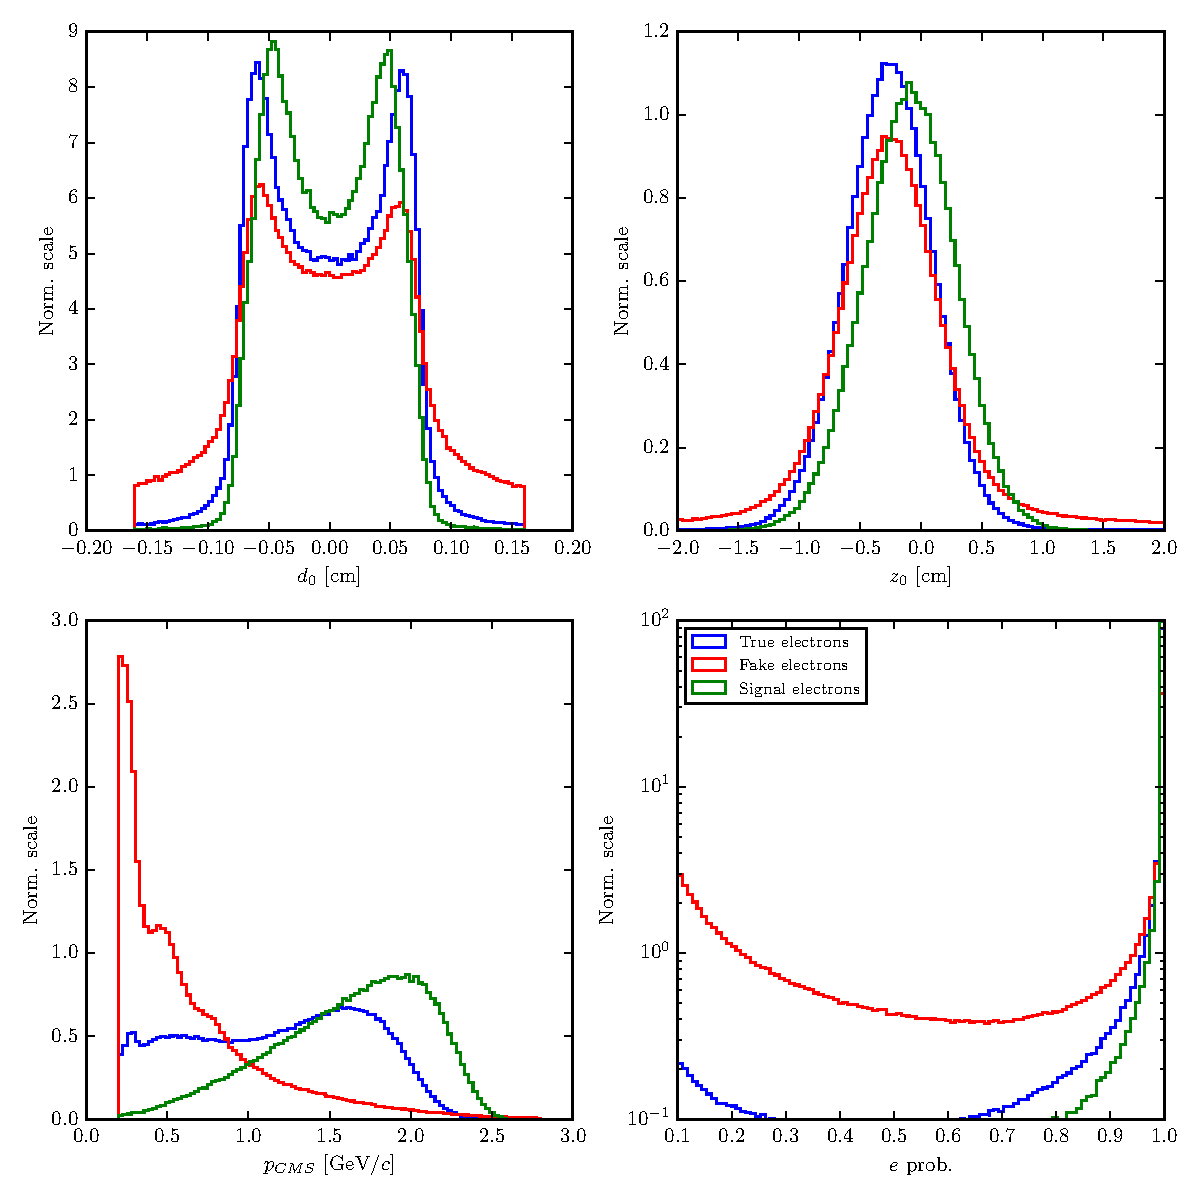
\includegraphics[scale=1]{fig/FSP_e_vars}
\caption{Caption}
\end{figure}

\begin{figure}[!h]
\centering
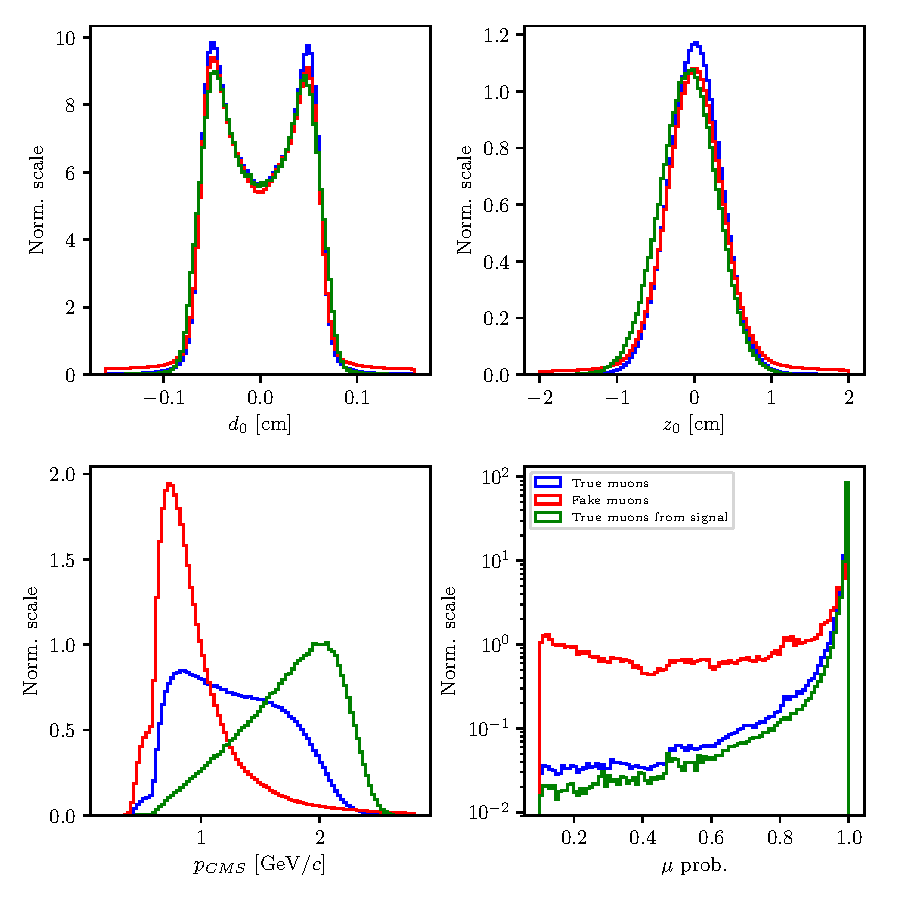
\includegraphics[scale=1]{fig/FSP_mu_vars}
\caption{Caption}
\end{figure}

Based on the first plots, we can define a set of cuts:
\begin{itemize}
\item $\vert d_0 \vert < 0.1\e{cm}$,
\item $\vert z_0 \vert < 1.5\e{cm}$,
\item $p_{LAB} > 0.6\e{GeV}/c$ and $p_{CMS} \in [0.4,\,2.6]~\e{GeV}/c$ for electrons,
\item $p_{CMS} \in [0.6,\,2.6]~\e{GeV}/c$ for muons,
\end{itemize}

where the $p_{LAB}$ momentum cut for the electron case is chosen to discard a region with a sharp jump, which is assumed to come from sources like hard coded values in Belle software.

With this selection we can now determine the optimal PID cuts for electrons and muons, where we optimize with the standard definition of \textit{figure of merit} (FOM)
\begin{equation}
\label{eq:fom}
FOM = \frac{S}{\sqrt{S+B}},
\end{equation} 
where $S$ represents number of signal and $B$ the number of background candidates.

\begin{figure}[!h]
\centering
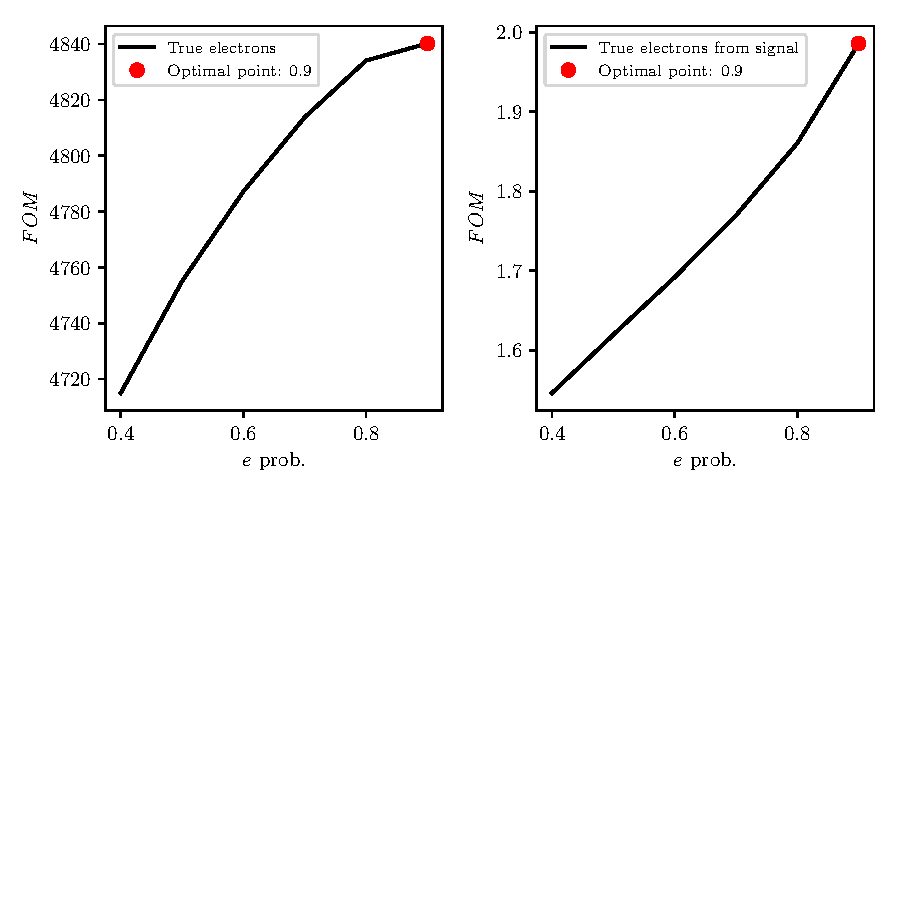
\includegraphics[scale=1]{fig/FSP_e_fom}
\caption{Caption}
\end{figure}

\begin{figure}[!h]
\centering
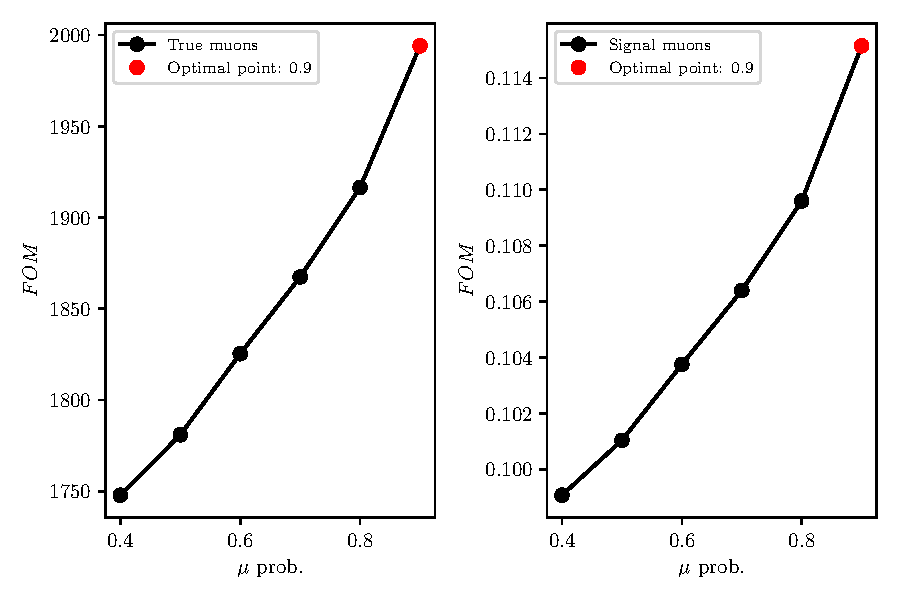
\includegraphics[scale=1]{fig/FSP_mu_fom}
\caption{Caption}
\end{figure}

We now define the PID cuts for leptons:
\begin{itemize}
\item $eID > 0.9$ for electrons,
\item $muID > 0.9$ for muons.
\end{itemize}

\subsubsection{Kaons}

For the case of kaons, the cuts are very similar

\begin{figure}[!h]
\centering
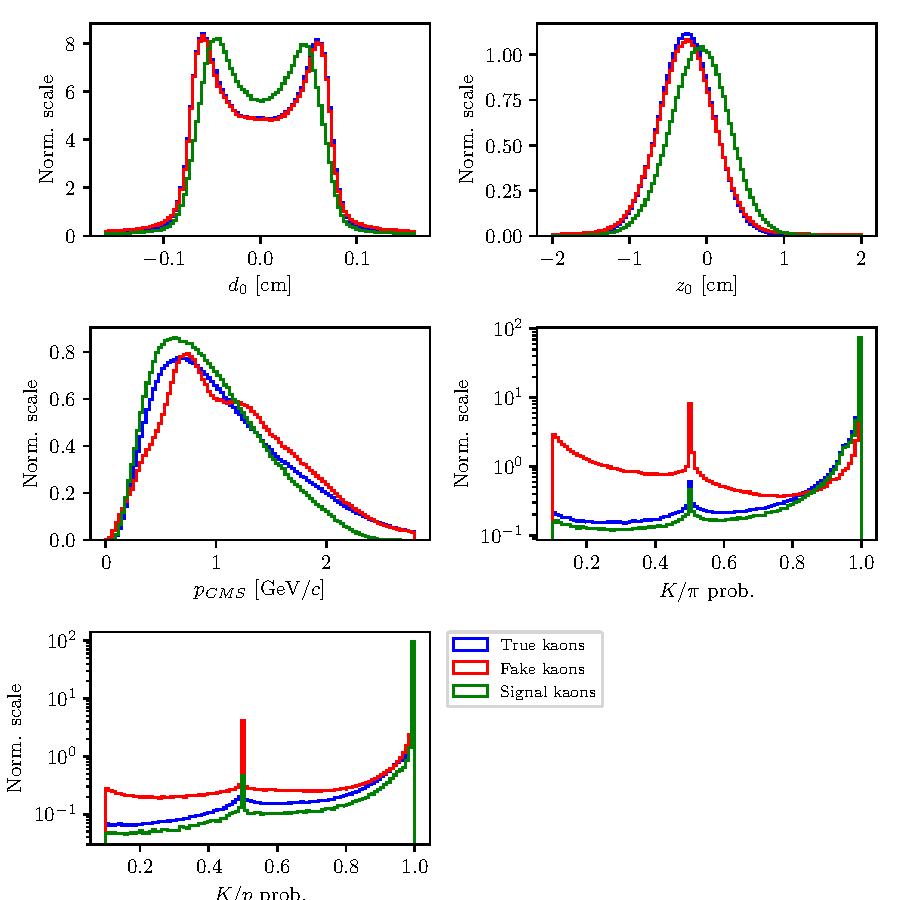
\includegraphics[scale=1]{fig/FSP_kaon_vars}
\caption{Caption}
\end{figure}

In the same manner we can define the cuts for kaons:
\begin{itemize}
\item $\vert d_0 \vert < 0.15\e{cm}$,
\item $\vert z_0 \vert < 1.5\e{cm}$,
\item $p_{CMS} \in [0,\,2.5]~\e{GeV}/c$.
\end{itemize}

The PID optimization in this case is taken in two steps. First we optimize the $K / \pi$ PID cut, and after that the $K/p$ PID cut.

\begin{center}
PLOT
\end{center}

The resulting PID cuts are then:
\begin{itemize}
\item $K/\pi > 0.7$,
\item $K/p > 0.3$.
\end{itemize}

\section{Combination of FSP particles}

With the reconstructed kaons and leptons we can now make appropriate combinations. Due to our inability to reconstruct the neutrino, we are only able, at this point, to reconstruct the $B$ mesons in the following two channels
\begin{align*}
B^+ &\to K^+ K^- e^+, \\
B^+ &\to K^+ K^- \mu^+.
\end{align*}

In order to further guarantee the proper selection of FSP particles in a arbitrary combination, we perform a vertex fit of the three tracks. $B$ mesons have a relatively long lifetime, so they travel and decay somewhere along the z-axis of the detector, due to the detector boost, so we perform the vertex fit with an \textit{iptube} constraint, which constrains the vertex to an elongated ellipsoid along beam direction. We demand that the fit converged apply a cut on the fit probability, which was optimized with the $FOM$ function.

The resulting PID cuts are then:
\begin{itemize}
\item $chiProb > 6\times 10^{-3}$.
\end{itemize}

With the neutrino being the only missing particle on the reconstructed side and with some assumptions, we can determine the angle between the direction of the reconstructed $B$ (denoted as $Y \to K K \ell$) and the true $B$, as
\begin{align}
\mathrm{p}_\nu &= \mathrm{p}_B - \mathrm{p}_{Y}, \\
\label{eq:massnu}
\mathrm{p}_\nu^2 = m_\nu^2 &= m_B^2 + m_Y^2 - 2E_BE_Y + 2\vec{p}_B \cdot \vec{p}_Y \approx 0, \\ 
\label{eq:cosby}
\cos \left(\theta_{BY}\right) &= \frac{2E_BE_Y - m_B^2 - m_Y^2}{2\vert \vec{p}_B \vert \vert \vec{p}_Y\vert},
\end{align} 

where all the energy and momenta above are calculated in the CMS frame. The mass of the neutrino equals 0 to a very good precision, so we used it in Eq. (\ref{eq:massnu}). In addition, we can substitute the unknown energy and momentum magnitude of the $B$ meson in Eq. (\ref{eq:cosby}), $E_B$ and $\vert \vec{p}_B \vert$, with quantities from the well known initial conditions
\begin{align}
E_B &= E_{CMS} / 2,\\
\vert \vec{p}_B \vert = p_B &= \sqrt{E_B^2 - m_B^2},
\end{align} 

where $E_{CMS}$ is the total energy of the $e^+e^-$ collision in the CMS frame. For the correctly reconstructed candidates, this variable  lies in the $[-1,1]$ region, while for the background candidates the values populate also the non-physical regions. Due to detector resolution effects, we impose the cut to somewhat larger values
\begin{itemize}
\item $\vert \cos \left(\theta_{BY}\right) \vert < 1.2$.
\end{itemize}

\begin{center}
PLOT
\end{center}

\section{Rest of event clean-up}

Due to the beam background in the detector, material interactions, or other processes, random tracks and clusters enter our event and get reconstructed as part of the physics process we want to study. These tracks and clusters are not interesting and further spoil the data we measure. In order to remedy this, we perform an extensive clean-up of the tracks and clusters in the ROE side, before calculating the four-momentum of the missing neutrino. The clean-up procedure is performed separately on tracks and clusters and uses multiple steps with multivariate analysis (MVA) algorithms in order to separate good tracks and clusters from the bad ones, which populate the ROE. Then for each ROE object, a ROE mask is created for tracks and clusters, which consists of boolean values for each track and cluster index in the ROE object, where the boolean value narrates the use of this track or cluster in the final calculations of the missing four-momentum.

A more detailed description of the ROE clean-up can be found in chapter X.

\section{Loose neutrino reconstruction}

As was already mentioned, the neutrinos in the event escape the detector, so we cannot determine it's four-momentum. However, due to the detectors geometry, which almost completely covers the full solid angle, and due to well known initial conditions of the $\Upsilon(4S)$ meson, it is possible to determine the kinematics of the neutrino by summing up all the FSP particles four-momenta in the event. This is known as the \textit{untagged} method.

The total missing four-momentum in the event can be determined as
\begin{align}
\mathrm{p}_{miss} &= \mathrm{p}_{\Upsilon(4S)} - \sum_i^{\mathrm{Event}}\left(E_i,\,\vec{p}_i \right),\\
\mathrm{p}_{miss} &= \mathrm{p}_{\Upsilon(4S)} - \left(\mathrm{p}_{Y} -\sum_i^{\mathrm{Rest~of~event}}\left(E_i,\,\vec{p}_i \right)\right).
\end{align}

where the summation runs over all charged and neutral particles in the event. We can define a new variable, $m_{miss}^2$, which is the square of the missing mass. If signal side neutrino is the only missing particle in the event, then this variable should be equal to zero
\begin{align}
\label{eq:nuold}
\mathrm{p}_\nu &= \mathrm{p}_{miss} = \left(E_{miss},\,\vec{p}_{miss} \right),\\
m_{miss}^2 &= \mathrm{p}_{miss}^2 = \mathrm{p}_{\nu}^2 = m_\nu^2 \approx 0.
\end{align}

Since the detector is not perfect, the distribution of the $m_{miss}^2$ variable has a non-zero width. Additionally, tails are introduced as soon as we have multiple missing neutrinos, other neutral undetected particles such as $K_L^0$, or simply missing tracks due to detection failure.

\begin{center}
PLOT
\end{center}

The main uncertainty in neutrino four-momentum, defined as in Eq. (\ref{eq:nuold}) comes from energy uncertainty. It is a common practice to substitute the missing energy with the magnitude of the missing momentum, since the momentum resolution is much better, thus redefining the neutrino four-momentum to
\begin{equation}
\label{eq:nunew}
\mathrm{p}_\nu = \left(\vert \vec{p}_{miss} \vert,\,\vec{p}_{miss} \right).
\end{equation}

With our newly defined neutrino four-momentum, we can add it to the four-momentum of the $Y(KK\ell)$ candidate to obtain the full $B$ meson four-momentum and calculate the traditional $M_{BC}$ and $\Delta E$ variables
\begin{align}
\Delta E &= E_B - E_{CMS}/2,\\
M_{BC} &= \sqrt{\left(E_{CMS}/2\right)^2 - p_B^2}.
\end{align}

Since the final fit will be performed on these two variables, we define two regions that will be used
\begin{itemize}
\item Fit region: $M_{BC} \in [5.1,\,5.3]\e{GeV}/c^2$ and $\Delta E \in [-1,\,1]\e{GeV}$,
\item Signal enhanced region: $M_{BC} \in [5.X,\,5.3]\e{GeV}/c^2$ and $\Delta E \in [-X,\,X]\e{GeV}$.
\end{itemize}

\begin{center}
PLOT
\end{center}

\section{$q^2$ calculation}

\chapter{Rest of event clean-up}

Continuing from X, the description of the ROE clean-up process is described here. 

\section{Setting up the MVA}

Training the MVA classifiers follows the same recipe for all the steps. For each step we run our $B$ meson reconstruction on Signal MC with a generic companion $B$ meson. This way the produced weight files are less likely to be dependent on the signal side and can be used also for untagged analyses of other decays. For every correctly reconstructed signal $B$ meson we save the necessary information for each MVA step (i.e. properties of ROE clusters). Only correctly reconstructed candidates are chosen here, to prevent leakage of information from the signal side to the ROE side.

For each cleanup-step a dataset of $2\times N$ was prepared for the training of "signal" against "background". The dataset for each case was split into 5 parts for reasons which are explained later on in the note. The Fast-BDT (FBDT) [] algorithm was used as the MVA method, where the following hyper-parameters were optimized with a grid search
\begin{itemize}
\item \texttt{nTrees}: the number of trees in the FBDT forest,
\item \texttt{nLevels}: the number of levels in each FBDT tree.
\end{itemize}

Figure X shows a graphical interpretation of the FBDT forest with \texttt{nTrees} and \texttt{nLevels}. In all cases the hyper-parameters were optimized with a grid search in the hyper-parameter space. Additionally, we perform a $k$-fold cross-validation ($k=5$) for each hyper-parameter set, where we cycle through the $5$ parts of the dataset and $4$ parts of the dataset are used for training, whereas the remaining part is used for validation. This minimizes the bias towards the validation sample when optimizing the hyper-parameters. Figure X shows a schematic procedure of a $k$-fold cross-validation.

\section{Clusters clean-up}

Generally speaking, most of the photons in $B$-physics should come from $\pi^0 \to \gamma \gamma$ decays. However, a lot of clusters are also created by photons coming from the beam background or interactions with the detector material. These photons add extra energy and momentum which we then measure.

In the first step of the clusters clean-up we train an MVA which recognizes good $\pi^0$ candidates. The output of this classifier is then applied to photons and represents a sort of a $\pi^0$ probability, which is used as an additional classifier variable in the next step of the clean-up, where we train an MVA to separate good photon clusters from bad ones.

\subsection{$\pi^0$ MVA training}

The dataset of $\pi^0$ candidates contains
\begin{itemize}
\item 387125 signal candidates,
\item 416019 background candidates,
\end{itemize}
where the definition of signal is that both photon daughters that were used in the reconstruction of the $\pi^0$ are actual photons and actual daughters of the particle, based on the MC truth. We use $\pi^0$ candidates from the converted $\pi^0$ particle list from Belle MC with the invariant mass in the range of $M \in [0.10,~0.16]\e{GeV}$ and perform a mass-constrained fit on all candidates, keeping only the cases where the fit converged. 

The input variables used in this MVA are
\begin{itemize}
\item $p$ and $p_{CMS}$ of $\pi^0$ and $\gamma$ daughters,
\item $P(\chi^2,NDF)$ of the mass-constrained fit, invariant mass and significance of mass before and after the fit,
\item angle between the daughter photons in CMS frame,
\item cluster quantities for each daughter photon
	\begin{itemize}
	\item $E_9/E{25}$,
	\item theta angle,
	\item number of hit cells in the ECL,
	\item highest energy in cell,
	\item energy error,
	\item distance to closest track at ECL radius.
	\end{itemize}
\end{itemize}

The classifier output variable is shown in Figure X.

\begin{center}
PLOT
\end{center}

The distributions for all input variables and their correlations for signal and background candidates can be found in Appendix X for all steps of the clean-up.


\subsection{$\gamma$ MVA training}

The dataset of $\gamma$ candidates contains
\begin{itemize}
\item 324781 signal candidates,
\item 333353 background candidates,
\end{itemize}
where the definition of signal is that the photon is an actual photon and that the related ECL cluster is related to a primary MC particle. This tags all photon particles from secondary interactions as background photons. We use $\gamma$ candidates from the converted $\gamma$ particle list from Belle MC. The $\pi^0$ probability information from the previous step is applied to all photon pairs which pass the same $\pi^0$ cuts as defined in the previous step. Since it's possible to have overlapping pairs, the $\pi^0$ probability is overwritten, if the new value is greater than the existing one, since this points to a greater probability of a correct $\pi^0$ combination.

The input variables used in this MVA are
\begin{itemize}
\item $p$ and $p_{CMS}$ of $\gamma$ candidates,
\item $\pi^0$ probability,
\item cluster quantities
	\begin{itemize}
	\item $E_9/E{25}$,
	\item theta angle,
	\item number of hit cells in the ECL,
	\item highest energy in cell,
	\item energy error,
	\item distance to closest track at ECL radius.
	\end{itemize}
\end{itemize}

The classifier output variable is shown in Figure X.

\begin{center}
PLOT
\end{center}

\subsection{Clusters clean-up optimization}

We now have the final weights for photon classification. We apply these weights to the photon particle list, coming from the generically decaying $B$ mesons with correctly reconstructed signal $B$ mesons on the other side. After applying the weights we optimize the cut based on the standard definition of the $FOM$. The cut optimization is shown in Figure X, with the optimal cut on the $\gamma$ classifier output at $X$.

\begin{center}
PLOT
\end{center}

Figure shows the LAB frame momentum of the photons before and after the cut in logarithmic scale. The signal efficiency and background rejection at this cut are
\begin{itemize}
\item Signal efficiency: $\epsilon_{SIG} = X$,
\item Background rejection: $1-\epsilon_{BKG} = X$.
\end{itemize}

\begin{center}
PLOT
\end{center}

\section{Tracks clean-up}


\section{Selection after clean-up}

\end{document}


